\chapter{Methodology}\label{chapter:3}
In this chapter, after a description of the main characteristics of the dataset, all the models which will be applied 
throughout the project are illustrated.
\section{Dataset}
These section is inspired by the description made available by the creators of the dataset 
at link \footnote{\url{https://github.com/m-chaves-inria/CIGAIA-argument-mining-war-ukraine/tree/main/documentation}}.


This dataset contains a corpus of news articles slected in social scientists in English and French from 2022 and 2023 
about the war in Ukraine. It is made of 1462 English articles (1.5 milion tokens) and 1865 French articles (1.8 milion 
tokens).


The articles were classified based on the year and on the topic (i.e. propaganda, terrorism, war crimes, etc.), 
which is different from their genre (i.e. speeches, interviews, opinion pieces, etc.). The articles were manually
reviewed to ensure that the full text was retrieved and they were cleaned to remove the irrelevant content like 
advertisements.

After creating the corpus, it needs to be annotated. The dataset is currently focus on intra-article annotation whose goal
is to identify claims, premises and relations between them in a single article. The description of these elements is given 
in section \ref{sec:am}. The annotators were first recruited via Prolific, a platform specific designed for connecting 
researchers with participants. The latter would then be sent to a platform called Label Studio, which is specifically 
designed for annotating text. However, the quality of the annotations was not satisfactory therefore the choice was to 
rely on a single expert annotator, who would create a gold-standard. The corpus is not currently entirely annotated, 
however the currently annotated corpus is deemed to be enough to pursue the goal of this project.
\subsection{Dataset statistics}
Table \ref{tab:argument_components} represents how the 1256 components are split between claims and premises across 30 articles for a total of 
26460 tokens. The longest of the analysed articles has 2379 tokens while the shortest article had 286 tokens. 

\begin{table}[htbp]
\centering


\begin{tabular}{lrr}
\toprule
\textbf{Component Type} & \textbf{Count} & \textbf{Percentage} \\
\midrule
Premise & 714 & 56.8\% \\
Claim & 542 & 43.2\% \\
\midrule
\textbf{Total} & \textbf{1,256} & \textbf{100.0\%} \\
\bottomrule
\end{tabular}
\caption{Distribution of argumentative components.}
\label{tab:argument_components}
\end{table}
As it is possible to see, premise tend to be more present than claims in the corpus as they are used in relation to claims (i.e. many premises can be 
linked to the same claims while the contrary is not usually true). 


Table \ref{tab:argument_relations} represents the distribution of the argumentative relations between claims and premises.

\begin{table}[htbp]
\centering
\begin{tabular}{lrr}
\toprule
\textbf{Relation Type} & \textbf{Count} & \textbf{Percentage} \\
\midrule
Support & 756 & 92.5\% \\
Attack & 61 & 7.5\% \\
\midrule
\textbf{Total} & \textbf{817} & \textbf{100.0\%} \\
\bottomrule
\end{tabular}
\caption{Distribution of argumentative relations}
\label{tab:argument_relations}
\end{table}

As it is possible to see from the table, the great majority of the argument components is in support of another component. This usually happens as news
articles rely on constructive argumentations  while disregarding adversial ones. 

The relation type and the component type are used to form the 439 connected components which together compose the dataset's argumentation graph.
The distribution of the components graph sizes is represented by figure \ref{fig:component_sizes}. As it is he distribution is right-skewed meaning that the majority of the graphs 
has a number of vertices lower than 5. The graph with the largest number of vertices had 27 of them.
\begin{figure}[htbp]
\centering
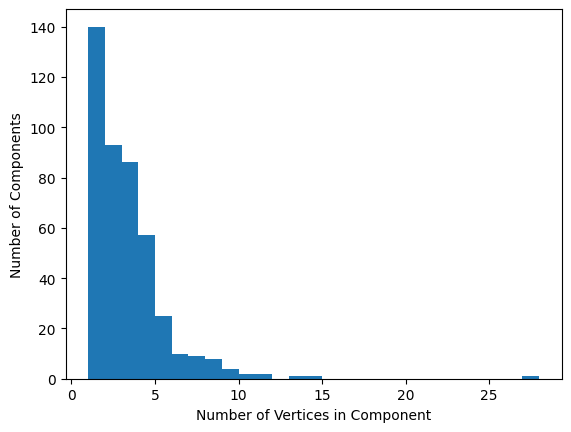
\includegraphics[width=0.7\textwidth]{img/distribution_component_sizes.png}
\caption{Distribution of argument component sizes in the annotated corpus}
\label{fig:component_sizes}
\end{figure}


The skewness in the distribution is probably due to large number of political speeches in the annotated dataset, 
which tend to have a simple structure to effectively address the audience. 